\chapter{数学建模 / 组会汇报，还要另做一套幻灯片}

\begin{notebox}
本章解决“论文一套、PPT 另起炉灶”的双重劳动：Beamer 让你用写论文的姿势做幻灯片，公式不用截图；TikZ 让示意图直接在文档里画，改起来不用开画图软件。
\end{notebox}

\painhead{烦恼}

“论文刚交完，导师说下周组会做个汇报 PPT。公式的截图糊成一团，改个符号要回 Word 重截，我是来做科研的不是来做美工的。”

\painhead{现象 · 这些场景你肯定见过}

\textbf{场景一}：数模论文里的核心公式要放进 PPT。你在 Word 公式编辑器里调好，截图，粘进 PowerPoint——投影到大屏幕上一放大，糊得像打了马赛克，评委眯着眼问“这个符号是 \ensuremath{\lambda} 还是人”。

\textbf{场景二}：技术路线图要画个“数据收集\ensuremath{\rightarrow}模型训练\ensuremath{\rightarrow}结果分析”的流程图。PowerPoint 的 SmartArt 套了半天模板，箭头总是对不齐，改一个框的位置，连着三根线要重新拖。

\textbf{场景三}：论文里的图要放进 PPT，尺寸一变，旁边的文字全跑位了。你花在“对齐”上的时间，比花在内容上的还多。

LaTeX 的回答：\textbf{幻灯片也是文档，公式图表直接复用你已经会的那些代码。} 论文里能写的，幻灯片里就能放。

\painhead{解决线路}

\subsection*{14.1 Beamer 最小可用框架}

新建文件，敲进去，引擎选 \textbf{XeLaTeX}，点绿色“排版”按钮：

\begin{lstlisting}
\documentclass{ctexbeamer}
\begin{document}

\titlepage

\begin{frame}{第一页正文}
你好，这是我的第一张幻灯片。
\end{frame}

\end{document}
\end{lstlisting}

编出来你会发现：屏幕比例 4:3，左上角有个进度条之类的东西——这就是 beamer，LaTeX 自带的幻灯片文档类。

\textbf{逐行拆解}：

\begin{itemize}
\setlength{\itemsep}{2pt}
\item \texttt{\textbackslash{}documentclass\{ctexbeamer\}}：beamer + 中文支持，一步到位。\textbf{写中文幻灯片，用 \texttt{ctexbeamer} 就完事了}，不用再折腾任何字体设置；
\item \texttt{\textbackslash{}titlepage}：标题页。不过它得知道标题是什么，所以完整的写法是下面这样；
\item \texttt{\textbackslash{}begin\{frame\}\{...\}} ... \texttt{\textbackslash{}end\{frame\}}：一页幻灯片。\texttt{frame} 就是“一页”，花括号里是这页的标题。你后面学的所有东西——公式、图、表——都往 frame 里塞。
\end{itemize}

完整版加上标题信息：

\begin{lstlisting}
\documentclass{ctexbeamer}
\title{基于机器学习的房价预测}
\author{张三}
\institute{某某大学 数学学院}
\date{\today}
\begin{document}

\titlepage

\begin{frame}{研究背景}
传统回归方法在高维数据上表现不佳。
\end{frame}

\end{document}
\end{lstlisting}

\texttt{\textbackslash{}title}、\texttt{\textbackslash{}author} 这些命令是不是很眼熟？对，跟第 3 章 \texttt{\textbackslash{}maketitle} 用的是同一套——这就是复用。

\subsection*{14.2 分节页和大纲：\texttt{\textbackslash{}tableofcontents} 的老朋友}

幻灯片也需要“第一章”“目录”。做法和正文完全一样，只是多了个“分节页”的常见操作：

\begin{lstlisting}
\documentclass{ctexbeamer}
\begin{document}

\begin{frame}{目录}
\tableofcontents
\end{frame}

\section{研究背景}

\begin{frame}{为什么研究这个问题}
数据量大，传统方法力不从心。
\end{frame}

\end{document}
\end{lstlisting}

\texttt{\textbackslash{}section} 在 beamer 里不产生正文标题，只出现在目录里。想让每个 section 开始时插一页高亮的分节页，先用土办法：section 前手动放一页 frame，里面写 \texttt{\textbackslash{}tableofcontents[currentsection]}——当前节高亮，其他变灰，答辩观感直接上一个档次。

\subsection*{14.3 主题：一句话换整套皮肤}

幻灯片长得好不好看，由主题决定。一行命令搞定：

\begin{lstlisting}
\usetheme{Madrid}
\end{lstlisting}

放在 \texttt{\textbackslash{}documentclass} 之后、\texttt{\textbackslash{}begin\{document\}} 之前。常用的内置主题速查：

\begin{table}[htbp]
\centering
\small
\begin{tabularx}{\linewidth}{@{}*{3}{>{\raggedright\arraybackslash}X}@{}}
\toprule
\textbf{主题名} & \textbf{风格} & \textbf{适合场合} \\
\midrule
\texttt{default} & 极简，啥装饰没有 & 不想分心的场合 \\
\texttt{Madrid} & 底部信息栏，稳重 & 组会、课程汇报（新手默认选它） \\
\texttt{Warsaw} & 顶部导航条，正式 & 学术答辩 \\
\texttt{Boadilla} & 低调清爽 & 课程作业展示 \\
\texttt{Singapore} & 顶部细进度条 & 内容多的长汇报 \\
\bottomrule
\end{tabularx}
\end{table}

另外提一嘴：\texttt{metropolis} 主题（\texttt{\textbackslash{}usetheme\{metropolis\}}）是社区公认颜值天花板，但需要额外装字体（Fira 系列），装不上就先跳过，Madrid 已经很体面了。

\begin{notebox}
\textbf{金句}：主题换得再花，内容才是幻灯片的灵魂——评委看的是你的模型，不是你的配色。
\end{notebox}

\subsection*{14.4 公式、图、表：直接复用正文的代码}

这是 beamer 最大的红利：第 6 章的公式、第 4 章的插图、第 7 章的表格，代码原封不动搬进 frame 就能用：

\begin{lstlisting}
\begin{frame}{核心模型}
损失函数定义为：
\begin{equation}
\mathcal{L} = \frac{1}{N}\sum_{i=1}^{N}\left(y_i - \hat{y}_i\right)^2
\end{equation}
其中 $N$ 为样本数量。

\begin{figure}
\centering
\includegraphics[width=0.6\textwidth]{figures/result.pdf}
\caption{预测结果对比}
\end{figure}
\end{frame}
\end{lstlisting}

公式是矢量渲染的，投影仪上放大多少倍都不糊——截图党从此毕业。

\subsection*{14.5 \texttt{\textbackslash{}pause}：够用即止}

想让内容一条一条出现，在 frame 里加 \texttt{\textbackslash{}pause}：

\begin{lstlisting}
\begin{frame}{本文三点贡献}
\begin{itemize}
\item 提出了新的特征工程方法 \pause
\item 设计了两阶段训练框架 \pause
\item 在三个数据集上验证了有效性
\end{itemize}
\end{frame}
\end{lstlisting}

每遇到一个 \texttt{\textbackslash{}pause}，这页就“翻”一次，内容分步出现。

\textbf{但是，听我一句劝：\texttt{\textbackslash{}pause} 用多了忘删是重灾区。} 尤其是打印讲义的时候——每页 PDF 变成四五页碎片。原则：一页最多一两个，用在“先给问题再给答案”这种真正需要悬念的地方。别把汇报做成翻页表演。

\subsection*{14.6 TikZ：示意图直接画在文档里}

SmartArt 的替代品。加载 \texttt{\textbackslash{}usepackage\{tikz\}}（放导言区），来一个“抄走就用”的三节点流程图：

\begin{lstlisting}
\documentclass{ctexbeamer}
\usepackage{tikz}
\usetikzlibrary{arrows.meta, positioning}
\begin{document}

\begin{frame}{技术路线}
\centering
\begin{tikzpicture}[
  node distance=1.5cm,
  box/.style={draw, rectangle, rounded corners,
              minimum width=2.8cm, minimum height=1cm, font=\small},
  arrow/.style={-{Stealth}, thick}
]
  \node[box] (a) {数据收集};
  \node[box, right=of a] (b) {模型训练};
  \node[box, right=of b] (c) {结果分析};
  \draw[arrow] (a) -- (b);
  \draw[arrow] (b) -- (c);
\end{tikzpicture}
\end{frame}

\end{document}
\end{lstlisting}

\textbf{逐行拆解}：

\begin{itemize}
\setlength{\itemsep}{2pt}
\item \texttt{\textbackslash{}usetikzlibrary\{arrows.meta, positioning\}}：加载两个工具库——前者提供好看的箭头样式，后者提供“放在某某右边”的定位语法；
\item \texttt{box/.style=\{...\}}：自定义一个叫 \texttt{box} 的节点样式——画框、圆角、最小宽高、小号字。定义一次，三个框共用，这就是“格式集中管理”的老思想；
\item \texttt{\textbackslash{}node[box] (a) \{数据收集\};}：放一个节点，样式是 \texttt{box}，给它起名叫 \texttt{(a)}，框里写字。\textbf{起名字是关键}——后面连线全靠名字；
\item \texttt{\textbackslash{}node[box, right=of a] (b) \{...\};}：第二个节点放在 \texttt{(a)} 的右边，间距 1.5cm（前面 \texttt{node distance} 定的）。你不用算坐标，TikZ 自己排；
\item \texttt{\textbackslash{}draw[arrow] (a) -- (b);}：从节点 a 画一根箭头到节点 b。
\end{itemize}

想加第三个箭头拐弯、加判断分支？改样式、加节点就行——线和节点都挂在“名字”上，挪框箭头自动跟。这就是它和 SmartArt 的本质区别：\textbf{你描述关系，它负责画。}

\subsection*{14.7 pgfplots：一条函数曲线的最小例子}

示意图用 TikZ，\textbf{数据图}（函数曲线、实验结果）用它的兄弟 pgfplots：

\begin{lstlisting}
\usepackage{pgfplots}   % 导言区
\end{lstlisting}

\begin{lstlisting}
\begin{frame}{模型收敛曲线}
\centering
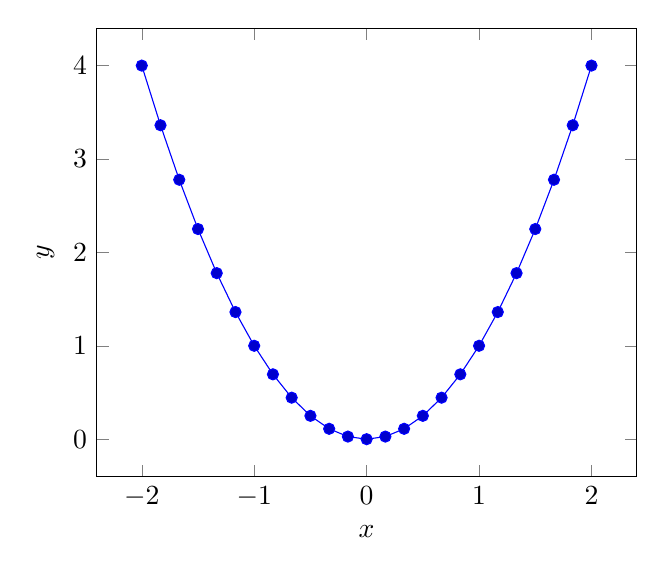
\begin{tikzpicture}
\begin{axis}[
  xlabel={$x$},
  ylabel={$y$},
  domain=-2:2
]
\addplot {x^2};
\end{axis}
\end{tikzpicture}
\end{frame}
\end{lstlisting}

\begin{itemize}
\setlength{\itemsep}{2pt}
\item \texttt{\textbackslash{}begin\{axis\}[...]}：开一个坐标系，方括号里写轴标签和取值范围；
\item \texttt{\textbackslash{}addplot \{x\textasciicircum{}2\};}：画 y = x² 的曲线。对，就是“打字”，跟写公式一个感觉。
\end{itemize}

和插图的取舍一句话说清：\textbf{示意图要经常改就用 TikZ 画，照片、软件导出的数据图还是老老实实插 PDF/PNG}——别用 TikZ 硬画你实验跑出来的折线图，那是给自己找事。

\painhead{Word 做法 vs LaTeX 做法 · 对照小结}

\begin{table}[htbp]
\centering
\small
\begin{tabularx}{\linewidth}{@{}*{3}{>{\raggedright\arraybackslash}X}@{}}
\toprule
\textbf{事项} & \textbf{Word / PowerPoint 做法} & \textbf{LaTeX 做法} \\
\midrule
论文公式搬进幻灯片 & 公式编辑器重打一遍或截图，投影发糊 & 代码原样复制，矢量渲染永不糊 \\
流程图 & SmartArt 套模板，拖线对齐半小时 & TikZ 节点+箭头，改字不动线 \\
换整套风格 & 换母版，元素跑得到处都是 & \texttt{\textbackslash{}usetheme\{\}} 一行换主题 \\
论文和幻灯片的内容同步 & 两套软件两份文件，改一处得改两处 & 同一套代码体系，复制即用 \\
分步出现动画 & 动画面板配半天 & \texttt{\textbackslash{}pause} 一个词（但也别贪多） \\
\bottomrule
\end{tabularx}
\end{table}

\painhead{翻车合集}

\begin{table}[htbp]
\centering
\small
\begin{tabularx}{\linewidth}{@{}*{3}{>{\raggedright\arraybackslash}X}@{}}
\toprule
\textbf{症状} & \textbf{原因} & \textbf{解法} \\
\midrule
中文显示乱码或空白 & 用了 \texttt{beamer} 而不是 \texttt{ctexbeamer}，或引擎没选 XeLaTeX & 文档类换 \texttt{ctexbeamer}，引擎选 XeLaTeX \\
内容超出页面，下面被裁掉 & 一页塞太多，beamer 不会自动缩 & 拆成两页 frame；宁可少放字 \\
演示时内容一页页蹦，收不住 & \texttt{\textbackslash{}pause} 加太多，忘了删 & 全局搜 \texttt{\textbackslash{}pause}，删到一页最多一两个 \\
\texttt{! I can't find file 'tikz.sty'} 之类 & 忘了 \texttt{\textbackslash{}usepackage\{tikz\}} 或写错库名 & 检查导言区，库名按本章原样抄 \\
图表编号显示"??" & 编译了一遍 & 再点一次排版按钮，老规矩（第 5 章讲过） \\
TikZ 节点重叠成一坨 & 忘了 \texttt{positioning} 库，或没用 \texttt{right=of} 语法 & 加 \texttt{\textbackslash{}usetikzlibrary\{positioning\}}，节点用相对定位 \\
\bottomrule
\end{tabularx}
\end{table}

\section*{练习}

\begin{enumerate}
\setlength{\itemsep}{2pt}
\item 用 \texttt{ctexbeamer} + \texttt{Madrid} 主题做一个 3 页的幻灯片：标题页、目录页、一页正文（随便写点你的课程内容），编译通顺；
\item 把你第 6 章练习里写过的一个行间公式原样搬进 frame，对比一下截图糊不糊——体会矢量渲染的爽；
\item 把 14.6 的三节点流程图抄下来编译成功，然后在“模型训练”和“结果分析”之间插一个新节点“模型调参”，体会加框加箭头有多省事；
\item 给 14.7 的例子改成画 \texttt{sin(x)} 曲线（domain 改成 \texttt{-3.14:3.14}），再给 \texttt{\textbackslash{}addplot} 加个选项 \texttt{[red, thick]} 看看效果；
\item \textbf{故意翻车题}：在一个 frame 里连加五个 \texttt{\textbackslash{}pause} 然后编译，数一数这一页在 PDF 里变成了几页——这就是“打印讲义惨案”的案发现场。以后用 \texttt{\textbackslash{}pause} 之前，先想想这张“残骸”。
\end{enumerate}

到这里，论文、模板、幻灯片你都能一个人包圆了。最后一章来一场综合实战：\textbf{从空白文件到一篇能交的小论文}，把全书学的十八般武艺串成一条流水线。
